%第3章


\section{スマートモビリティレジシステムの概要}

本節では,スマートモビリティレジシステムの目的,要求仕様及び概要を述べる.

まず,スマートモビリティレジシステムの目的としては既存の無人レジ店舗のような複雑で高価なシステムではなく,小規模や中規模の企業でも導入できる安価なスマートモビリティレジシステムの作成である.この目的を基にし,スマートモビリティ決済システムは,下記の3点の要求事項を満たす必要がある.

\begin{itemize}
\item 従来のセルフレジよりコストは抑えられる.
\item 既存の中小店でも導入が容易.
\item 従来のセルフレジより簡単な動作で決済まで行える.
\end{itemize}


上述の「従来のレジよりコストは抑えられる.」という評価軸には,カゴ90台を導入するコストと,登録機1台1,875,000円と精算機$2,750,000円\times7台$として,合わせておよそ21,125,000円\cite{super}とレジの店員分の人件費を合わせたコストを比べた際,よりコストを抑えられるかということである.また,上述の「従来のレジより簡単な動作での決済まで行える.」という要求項目は,従来の店員のように,商品を手に取り,バーコードリーダで商品のバーコードを読み取り,カゴへ入れるという動作と全く同じ動作をしないということである.

以上の要求事項を満たすためには,本研究では,WebカメラとRaspberry Pi,各種センサを各買い物カゴに設置し,従来のセルフレジやセミセルフレジに比べて安価かつ簡単に決済できるスマートモビリティレジを提案する.

本研究において対象として設定したスーパーマーケットを下記の表\ref{taisho}に示す.


\begin{table}[htb]
\begin{center}
\caption{対象スーパーマーケット}
\begin{tabular}{|l|c|c|c|} \hline
店舗 & 売場面積(平方メートル) & レジ台数 & カゴ数 \\ \hline
小規模店舗,中規模店舗 & 1,200 & 7台 & 90個 \\ \hline
\end{tabular}
\label{taisho}
\end{center}
\end{table}


表\ref{taisho}を対象として設定した理由を下記に述べる.本研究では小規模店舗と中規模店舗のスーパーマーケットを対象とする.小規模店舗は「売場面積$800m^2未満」あるいは「売場面積800m^2~1,200m^2未満」の店舗,中規模店舗は「売場面積800m^2~1,200m^2未満」または「売場面積1,200m^2~1,600m^2未満」の店舗を指す\cite{super}.本研究では,小規模店舗と中規模店舗の平均である,売り場面積1,200m^2の店舗を本研究の対象の店舗とする.売場面積1,000m^2あたりレジ台数は,平均5.7台のため,対象の売場面積1,200m^2の店舗ではレジ台数平均6.84台と仮定できる\cite{super}.四捨五入してレジ台数は7台とし,対象のレジ台数とする.また,売場面積が1,200m^2~1,600m^2$のスーパーマーケットの場合,平日レジ一台あたり一日客数は中央値として225.5人である\cite{super}.なお,平均営業時間は12.3時間のため,一時間あたり約18人の客がレジを使用すると予測できる\cite{super}.1人につき1個のカゴを使用しピーク時等の客入りを5倍,かつ店内に滞在する時間を1人につき1時間と仮定すると,約90個のカゴが必要と仮定した.


本研究で提案するシステムを使用する流れを図\ref{summary1}に示す.


\begin{figure}[htbp]
\centering
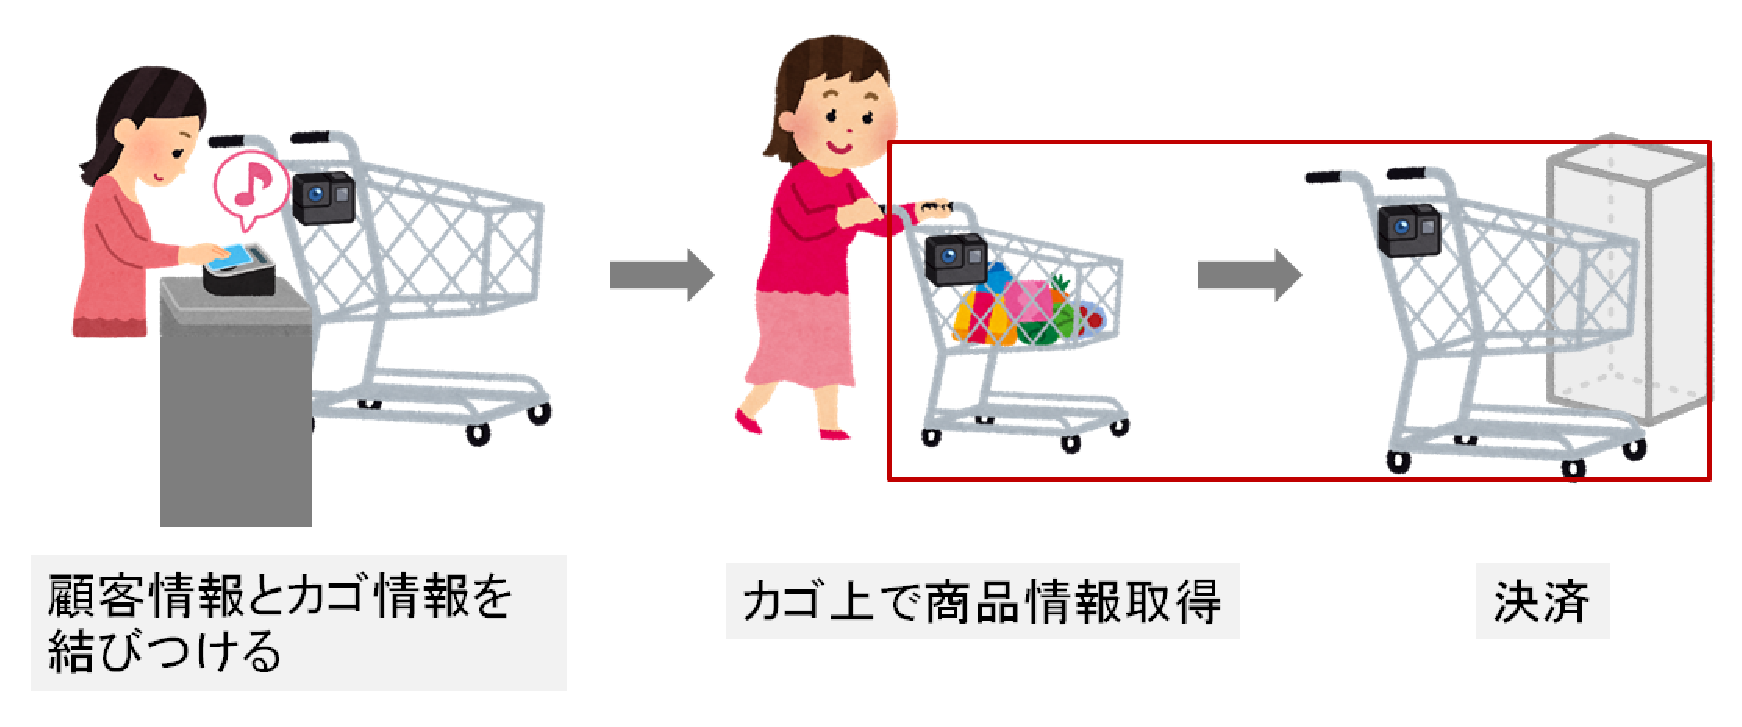
\includegraphics[width = 15cm]{./picture/summary1.eps}
\caption{商品識別システム全体の流れ}
\label{summary1}
\end{figure}



まず,ユーザが買い物カゴを取って,顧客情報をカゴ情報と結び付ける.その後,顧客はカゴを持ち歩きながら商品を選んで,購入しようとした商品をカゴに入れる.その際,センシング技術を用いて,カゴ上に組み込まれた商品識別装置(カメラ等)による商品情報を取得しサーバへ情報を送信する.買い物を終える際は,カゴを返却するだけで決済が行われる流れとなる.本研究ではスマートモビリティレジシステム全体の流れについて設計を行ったが,最終的には,優先度が高い機能とした図\ref{summary1}に示す赤枠に囲まれる,カゴ上で商品情報を取得し決済を行う部分を開発対象とした.上記範囲のスマートモビリティレジシステムのイメージ図を以下の図\ref{summary2}に示す.


\begin{figure}[htbp]
\centering
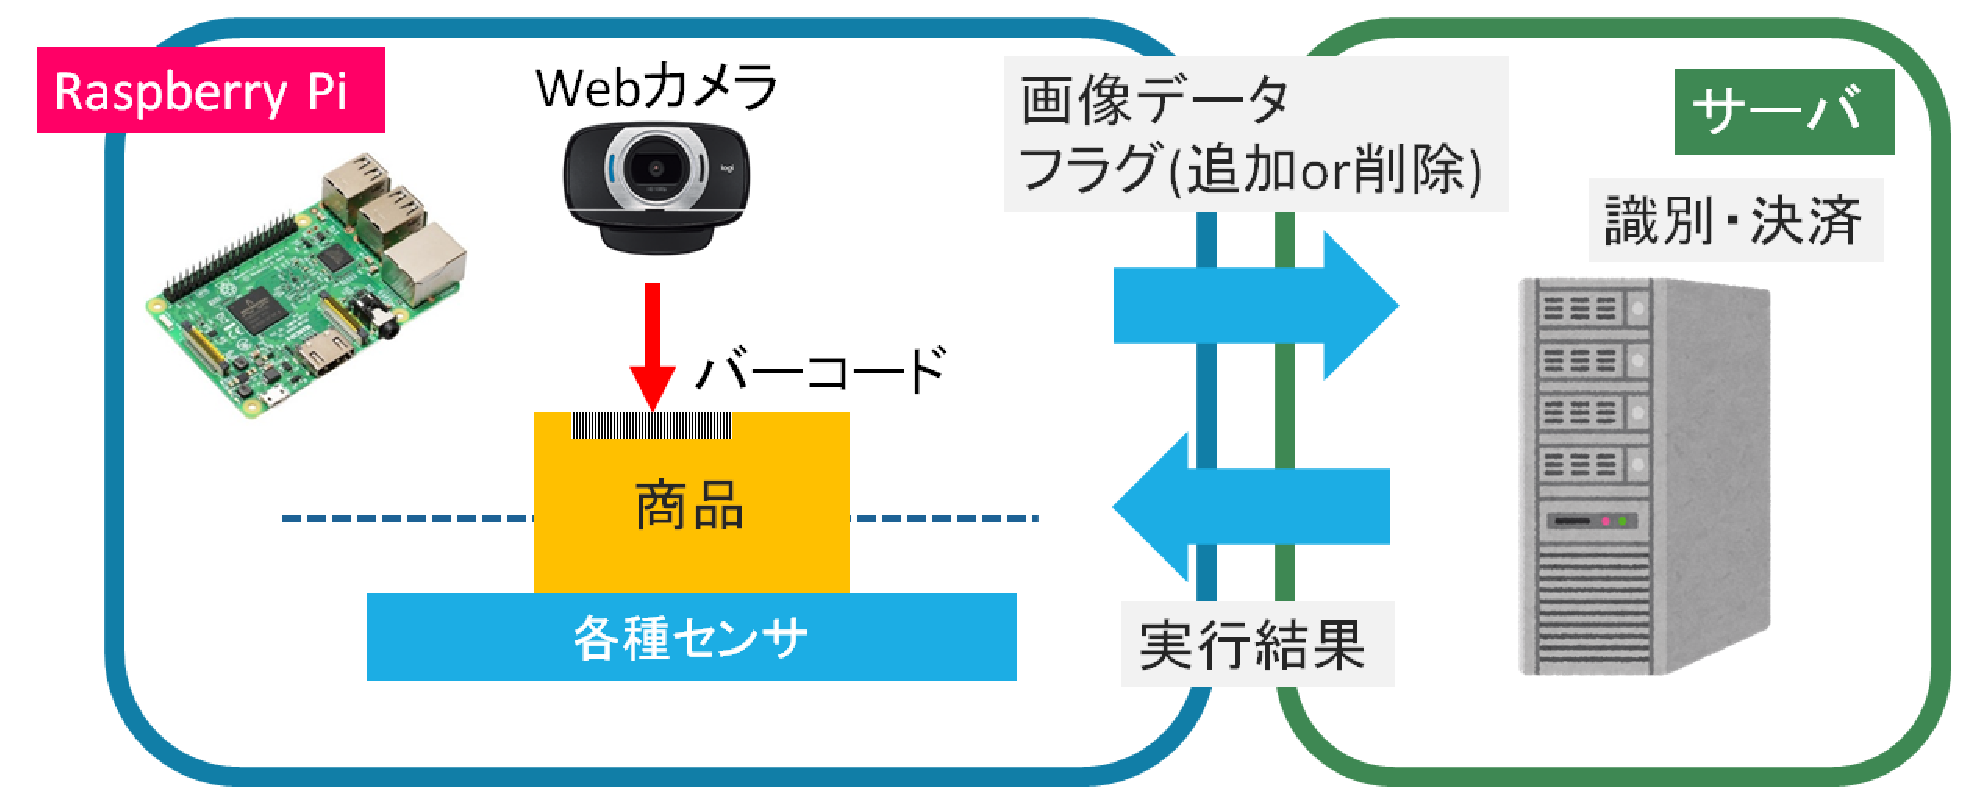
\includegraphics[width = 15cm]{./picture/summary2.eps}
\caption{スマートモビリティレジシステムのイメージ図}
\label{summary2}
\end{figure}


スマートモビリティレジシステムは識別・決済等を行うサーバ側,Raspberry PiとWebカメラ,および各種センサを設置した買い物カゴであるエッジ側(モビリティショッピング端末)の2つのパートで構成される.商品を各種センサが検知した際,Webカメラで商品のバーコードを撮影し,画像データ等をサーバへ送信する.サーバでは取得した商品のバーコード情報等を識別し,カゴに入れた商品の種類,金額,賞味期限,入れる時間などの情報を決済システムに一時的に保存し,仮登録する.ユーザはショッピングが終了する時点(例えば,決済ゲージを通る)に仮登録した商品の最終決済を行う.本システムの開発は,サーバ側を段原丞治が,モビリティショッピング端末を真鍋樹が担当した.